\documentclass[12pt]{article}
\usepackage{graphicx}
\usepackage{amsmath}
\usepackage{booktabs}
\usepackage[margin=1in]{geometry}
\usepackage{float}

\title{Report: Portfolio Optimization and Performance vs NIFTY 50}
\author{Debarshi Chakraborty \& Rudrajit Dey}

\begin{document}

\maketitle

\section{Introduction}

This study applies Markowitz Modern Portfolio Theory (MPT) to a selection of 10 NSE-listed stocks.
The objective is to:

Construct the Minimum Variance Portfolio (MVP) using historical data,

Allocate an initial investment of Rs 100,000,

Backtest performance against the NIFTY 50 index,

Evaluate whether MPT yields superior risk-adjusted performance.

\section{Data Collection}

Stocks: HDFC Bank, ITC, TCS, Reliance, Coal India, Infosys, Bajaj Finance, Asian Paints, L\&T, BEL.

Data Source: Yahoo Finance (yfinance).

Period: 30 Aug 2023 – 30 Aug 2025.

Dataset length: 494 daily observations.

Data was split:

First half (248 days) $\rightarrow$ used to estimate expected returns ($\boldsymbol{\mu}$) and covariance ($\boldsymbol{\Sigma}$).

Second half (246 days) $\rightarrow$ used for out-of-sample testing.

\section{Methodology}
\subsection{Returns}

Daily percentage returns were computed:

\[
r_{i,t} = \frac{P_{i,t} - P_{i,t-1}}{P_{i,t-1}}
\]

\subsection{Estimation}

Expected returns ($\boldsymbol{\mu}$): vector of daily mean returns.

Covariance matrix ($\boldsymbol{\Sigma}$): captures variance and correlation between assets.

Inverse covariance ($\boldsymbol{\Sigma}^{-1}$): used in optimization.

\subsection{Portfolio Weights}

MVP weights were derived as:

\[
\mathbf{w}_{MVP} = \frac{\boldsymbol{\Sigma}^{-1} \mathbf{1}}{\mathbf{1}^T \boldsymbol{\Sigma}^{-1} \mathbf{1}}
\]

Investment: Rs 100,000 allocated proportionally to weights.

\subsection{Mean-Variance Frontier}

For any target return $y$, the portfolio variance is:

\[
\sigma^2(y) = \frac{C}{D}\left(y - \frac{B}{C}\right)^2 + \frac{1}{C}
\]

where

\[
A = \boldsymbol{\mu}^T \boldsymbol{\Sigma}^{-1} \boldsymbol{\mu}, \quad
B = \boldsymbol{\mu}^T \boldsymbol{\Sigma}^{-1} \mathbf{1}, \quad
C = \mathbf{1}^T \boldsymbol{\Sigma}^{-1} \mathbf{1}, \quad
D = AC - B^2
\]

$\boldsymbol{\mu}$ = expected returns vector

$\boldsymbol{\Sigma}$ = covariance matrix of returns

$\mathbf{1}$ = vector of ones

This formula gives the parabolic frontier in mean-variance space.

\subsection{Mean-Std Dev Frontier}

Replacing variance $\sigma^2$ with standard deviation $\sigma$, we get the hyperbolic frontier:

\[
\sigma(y) = \sqrt{\frac{C}{D}\left(y - \frac{B}{C}\right)^2 + \frac{1}{C}}
\]

This is more intuitive to investors, since risk is measured in standard deviation rather than variance.

\subsection{Zero-Covariance Portfolio Relationship}

If portfolio $p$ has expected return $b_p$, then the return of portfolio $q$, which is uncorrelated with $p$, is:

\[
b_q = \frac{B}{C} - \frac{D}{C^2(b_p - B/C)}
\]

This illustrates how two portfolios on the frontier can be constructed to be mutually uncorrelated.

\section{Results}
\subsection{Efficient Frontier}

Theoretical risk–return trade-off, with the MVP marked.
\begin{figure}[H]
    \centering
    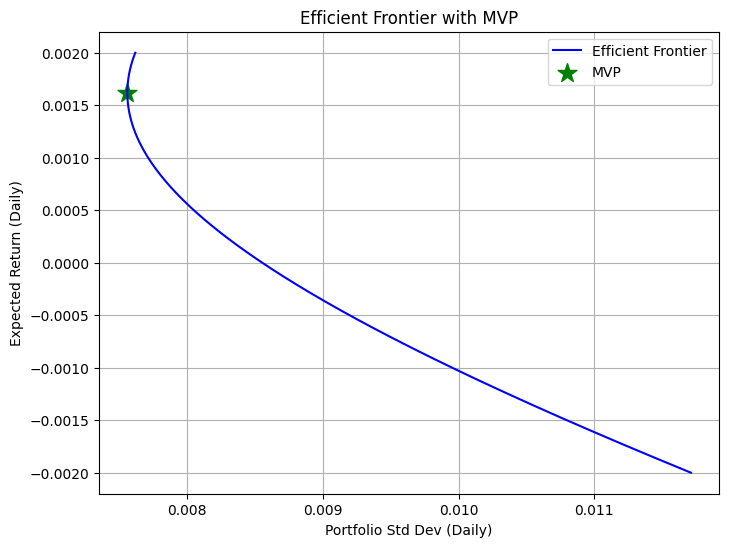
\includegraphics[width=0.8\textwidth]{5.png}
    \caption{Efficient Frontier with MVP}
    \label{fig:eff_frontier}
\end{figure}

\subsection{Mean-Variance and Mean-Std Dev Frontier}

\begin{figure}[H]
    \centering
    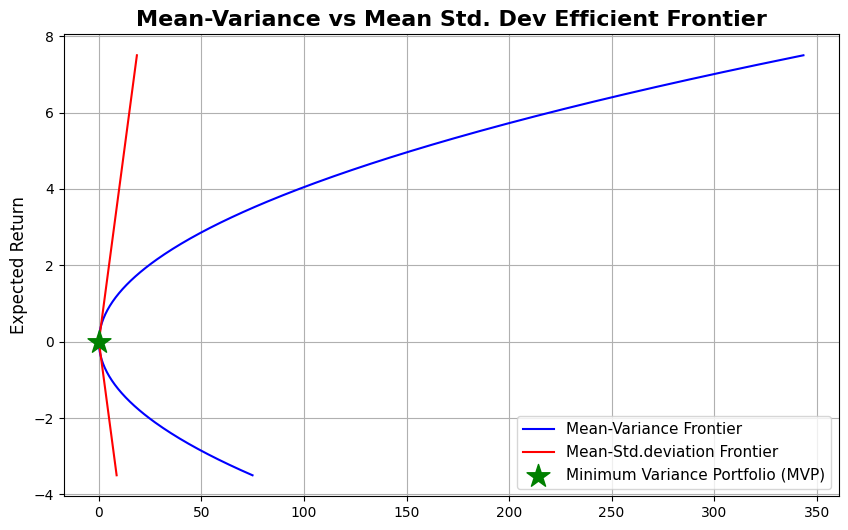
\includegraphics[width=0.8\textwidth]{1.png}
    \caption{Mean-Variance vs Mean-Std Dev Efficient Frontier}
    \label{fig:frontier_comparison}
\end{figure}

This figure shows both:

The parabolic frontier (Variance),

The hyperbolic frontier (Std Dev),

The Minimum Variance Portfolio (MVP) marked with a green star.

\subsection{Zero-Covariance Relationship}

\begin{figure}[H]
    \centering
    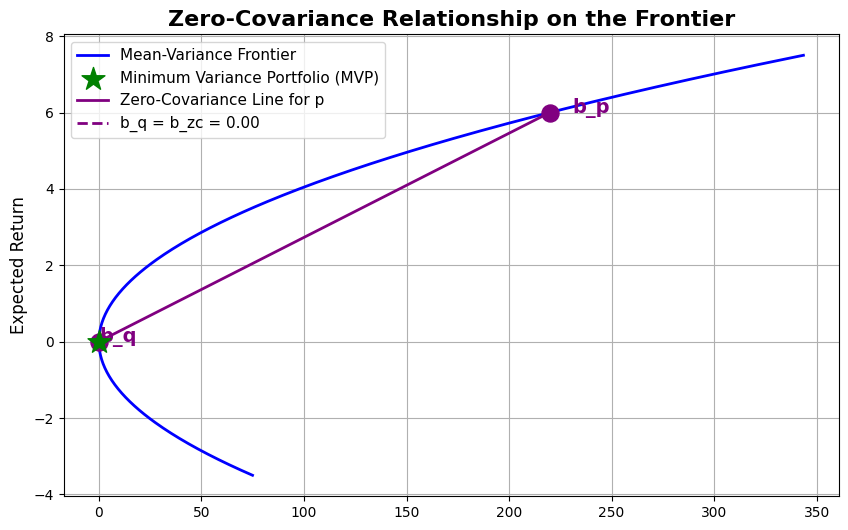
\includegraphics[width=0.8\textwidth]{2.png}
    \caption{Zero-Covariance Relationship on the Frontier}
    \label{fig:zero_covariance}
\end{figure}

This figure highlights:

The MVP,

A chosen portfolio $p$ with return $b_p$,

Its zero-covariance counterpart $q$ with return $b_q$.

Together, these illustrate the geometric properties of the frontier.

\subsection{Portfolio Allocation}

Final MVP allocation (weights):

HDFCBANK.NS: 21.2\%

ITC.NS: 0.6\%

TCS.NS: –1.0\%

RELIANCE.NS: –0.4\%

COALINDIA.NS: 17.1\%

INFY.NS: 6.5\%

BAJFINANCE.NS: 26.1\%

ASIANPAINT.NS: $\approx$0\%

LT.NS: 12.4\%

BEL.NS: 17.5\%

\begin{figure}[H]
    \centering
    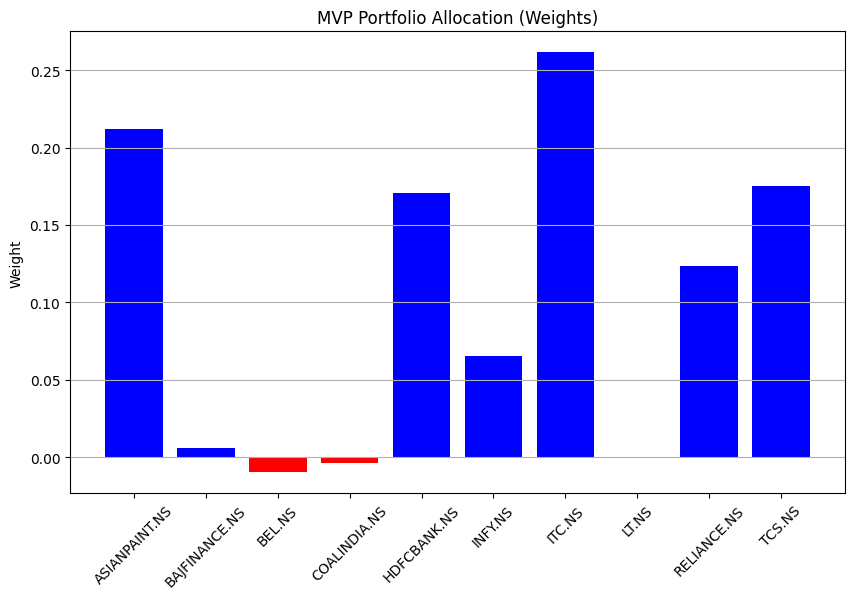
\includegraphics[width=0.8\textwidth]{3.png}
    \caption{Bar Chart of MVP Portfolio Weights}
    \label{fig:weights}
\end{figure}

\subsection{Performance (Out-of-Sample, 2024-2025)}

Comparison of MVP vs NIFTY 50:

\begin{table}[H]
    \centering
    \begin{tabular}{lrr}
        \toprule
        Metric & Your MVP & NIFTY 50 \\
        \midrule
        Total Return (\%) & –13.6\% & –1.4\% \\
        Annualized Return (\%) & –13.3\% & –0.6\% \\
        Annualized Volatility (\%) & 13.1\% & 13.3\% \\
        Sharpe Ratio & –1.09 & –0.05 \\
        Max Drawdown (\%) & –20.7\% & –15.8\% \\
        Final Value (Rs 100k) & Rs 86,446 & Rs 98,587 \\
        \bottomrule
    \end{tabular}
    \caption{Performance Comparison}
    \label{tab:performance}
\end{table}

\begin{figure}[H]
    \centering
    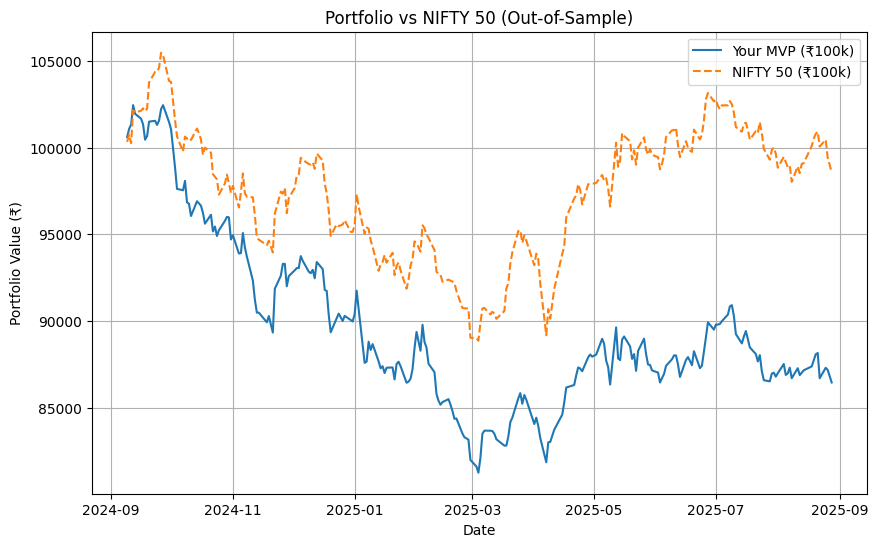
\includegraphics[width=0.8\textwidth]{4.png}
    \caption{Cumulative Value Curve: MVP vs NIFTY 50}
    \label{fig:cumulative}
\end{figure}

\section{Discussion}

MVP underperformed relative to NIFTY 50 in the test period.

Despite having similar volatility, MVP produced significantly lower returns.

The Sharpe ratio was highly negative, showing poor risk-adjusted performance.

Reason:

MVP focuses only on variance minimization, not return maximization.

Estimated returns/covariance are unstable with limited data.

Short positions (TCS, Reliance) worsened performance.

\section{Conclusion}

We successfully applied MPT and constructed the MVP.

Out-of-sample results showed MVP lost $\sim$13.6\% vs NIFTY's –1.4\%.

The study highlights the gap between theory and practice:

Optimization improves understanding,

But naive application may yield worse results than benchmarks.

\end{document}